\graphicspath{{images/act_1.1.2/}}
\subsubsection{Only damping}
The movements of ur5 robot is controlled with a derivative impedance control method at joint level. Thus, control law can be computed as 
\begin{equation}
	\boldsymbol{\tau}
	= \mathbf{D_{des} \dot{e}},
	\label{eq:articular_Di}
\end{equation}
\noindent where $\mathbf{e}=\mathbf{q_{des} - q}$ is joint position error, and $\mathbf{D_{des}}$ is desired damping. 

Figure \ref{fig:act1.1.2_tau_vs_q}-\ref{fig:act1.1.2_tau_vs_ddq} show relation between external force ($\tauext$) and joint configuration ($\jointconfiguration$) using control law \eqref{eq:articular_Di} with $\mathbf{D_{des}}=10\eye$ $\mathrm{\frac{N.m.s}{rad}}$. In these figures, the joints present different dynamic behaviors despite having the same control law. This is because the robot configuration generates different inertial and gravitational effects on each joint. In this context, the first three joints $(\mathrm{q_1, q_2, q_3})$ are most affected by the weight of ur5 robot. For this reason, the last three joints $(\mathrm{q_4, q_5, q_6})$ have similar graphs and maintain the dynamic relationship with the external force $\tauext$; while the first three $(\mathrm{q_1, q_2, q_3})$ have different graphs because the control law does not compensate for inertial and gravitational effects. Finally, the dynamic relationship of the last joint ($\mathrm{q_6}$) is a circle in position, line in velocity and circle in acceleration. This can be analyzed in more detail with graphs of joint configuration and external torque versus time. 

Figure \ref{fig:act1.1.2_tau_and_q}-\ref{fig:act1.1.2_tau_and_ddq} show joint configuration ($\jointconfiguration$) and external torque ($\tauext$) versus time. In these figures, joint configuration and external torque were normalized to obtain the same range of values\normalizenote. First, Figure \ref{fig:act1.1.2_tau_and_q} shows that $\tauext$ leads $\mathrm{q_6}$ by $90^{\circ}$. In this context, $\tauext$ describes a $\sin{(\cdot)}$ function whereas $\mathrm{q_6}$ describes a -$\cos{(\cdot)}$ function. Hence, the circular relationship between $\mathrm{q_6}$ and $\tauext$, described in Figure \ref{fig:act1.1.2_tau_vs_q}, can be justified. Second, Figure \ref{fig:act1.1.2_tau_and_dq} shows that $\mathrm{\dot{q}_6}$ is aligned in phase with $\tauext$. Hence, the line relationship between $\mathrm{\dot{q}_6}$ and $\tauext$, described in Figure \ref{fig:act1.1.2_tau_vs_dq}, can be justified. Finally, Figure \ref{fig:act1.1.2_tau_and_ddq} shows that $\mathrm{\ddot{q}_6}$ leads $\tauext$ by $90^{\circ}$. In this context, $\tauext$ describes a $\sin{(\cdot)}$ function whereas $\mathrm{\ddot{q}_6}$ describes a $\cos{(\cdot)}$ function. Hence, the circular relationship between $\mathrm{\ddot{q}_6}$ and $\tauext$, described in Figure \ref{fig:act1.1.2_tau_vs_ddq}, can be justified.

The relation between $\tauext$ and $\mathrm{q_6}$ could be analyzed using Laplace. It can be assumed, without generating large calculation errors, that the inertial and gravitational effects are close to $0$ for the last joint ($\mathrm{q_6}$). Thus, simplified dynamic equation of $\mathrm{q_6}$ is $\ddot{q}=D_\mathrm{des}\dot{q}_\mathrm{des} - D_\mathrm{des}\dot{q} + \tau_\mathrm{ext}$. Then, representing in Laplace
\begin{equation*}
\dot{q}_{6}(s) = \frac{D_\mathrm{des} \dot{q}_\mathrm{des}(s)}{s + D_\mathrm{des}} + \frac{1}{s + D_\mathrm{des}} \tau_\mathrm{ext}(s), 
\end{equation*}
where $\frac{D_\mathrm{des} \dot{q}_\mathrm{des}(s)}{s + D_\mathrm{des}}$ just add a constant value to the output signal and $G=\frac{1}{s + D_\mathrm{des}}$ is a filter that does not modify frequency of input signal. Hence, considering $\tau_\mathrm{ext}= 20\sin{(2\pi t)}$ as input, the output signal will be $\mathrm{\dot{q}_6}\approx 1.70\sin{(2\pi t)}$. Then, the linear relationship between $\mathrm{\dot{q}_6}$ and $\tau_\mathrm{ext}$ could be justified. Second, time-derivative of $\mathrm{\dot{q}_6}$ could be approximated as $\mathrm{\ddot{q}_6} \approx 10.6\cos{(2\pi t)}$. Then, circular relationship between $\mathrm{\ddot{q}_6}$ and $\tau_\mathrm{ext}$ could be justified. 

\begin{figure}
\centering
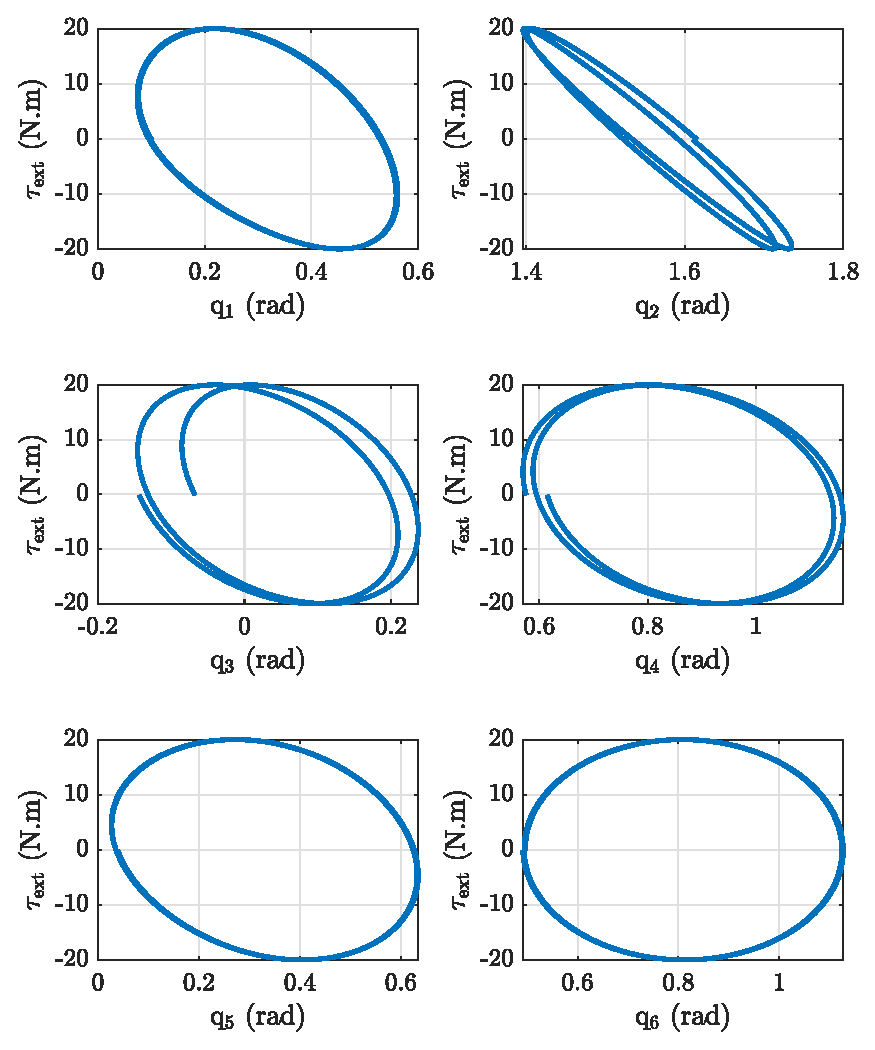
\includegraphics{external_torque_vs_joint_position.eps}
\caption{Dynamic relation between external torque ($\tauext$) and joint positions ($\mathbf{q}$) using proportional impedance control \eqref{eq:articular_Di} with $\mathbf{D_{des}}=10\eye$ $\mathrm{\frac{N.m.s}{rad}}$.}
\label{fig:act1.1.2_tau_vs_q}
\end{figure}

\begin{figure}
\centering
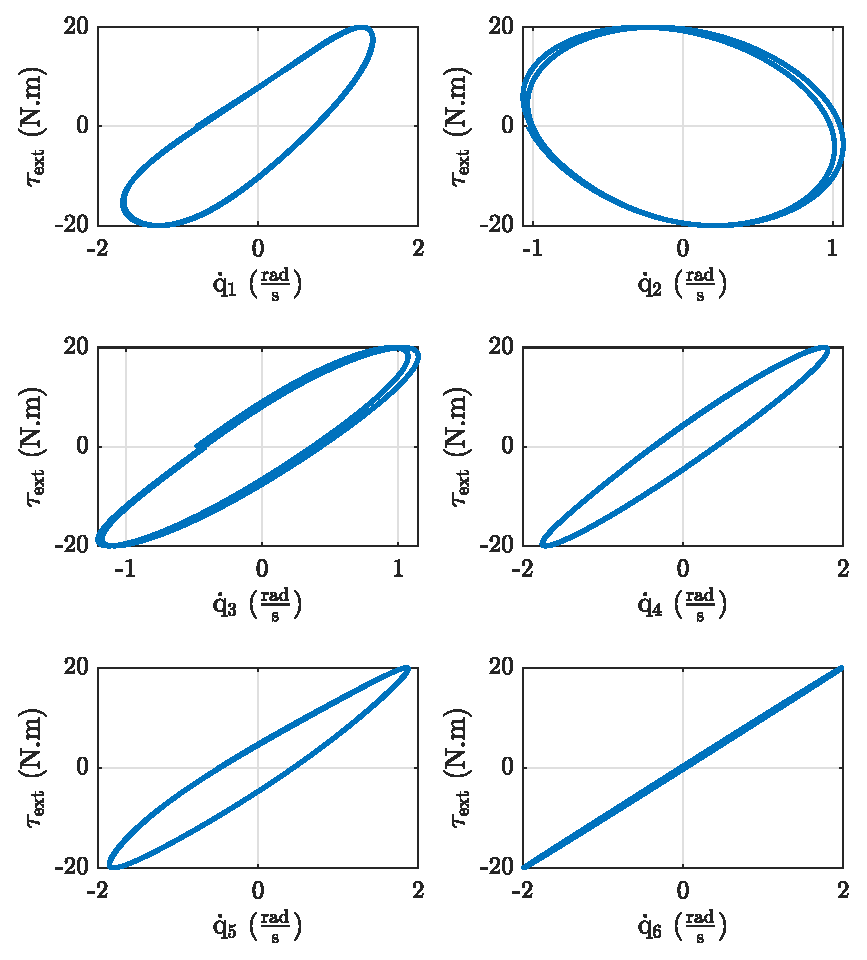
\includegraphics{external_torque_vs_joint_velocity.eps}
\caption{Dynamic relation between external torque ($\tauext$) and joint velocities ($\mathbf{\dot{q}}$) using proportional impedance control \eqref{eq:articular_Di} with $\mathbf{D_{des}}=10\eye$ $\mathrm{\frac{N.m.s}{rad}}$.}
\label{fig:act1.1.2_tau_vs_dq}
\end{figure}

\begin{figure}
\centering
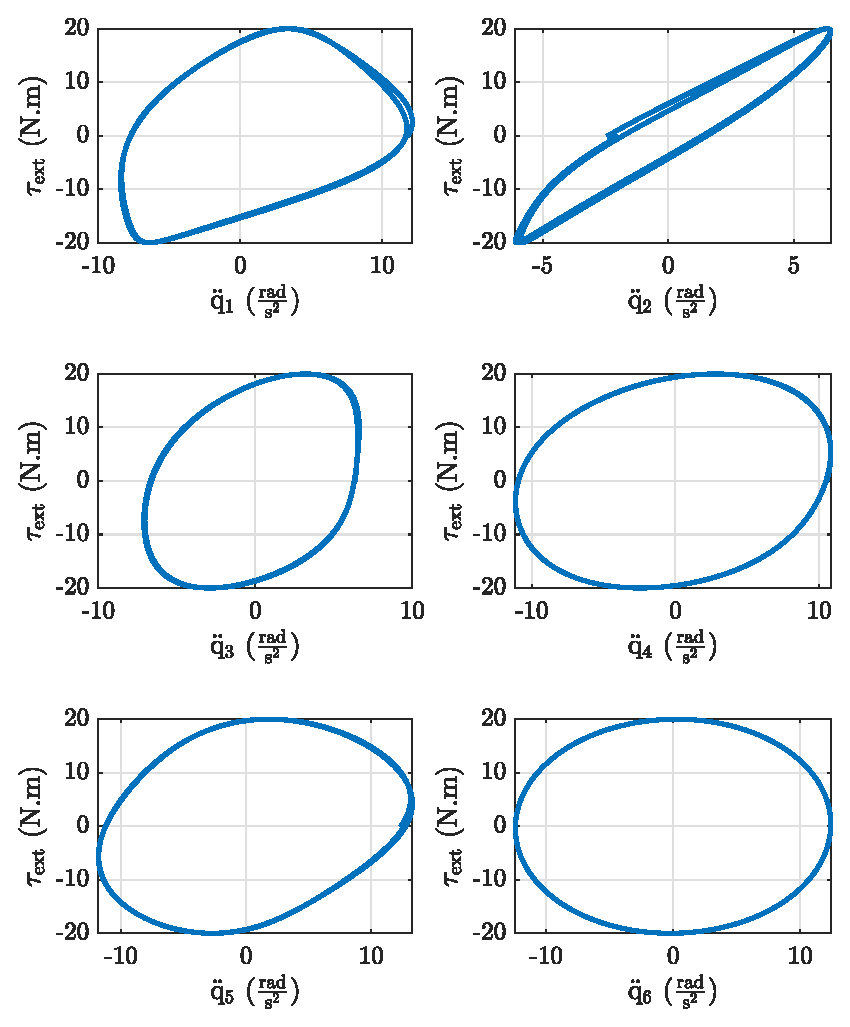
\includegraphics{external_torque_vs_joint_acceleration.eps}
\caption{Dynamic relation between external torque ($\tauext$) and joint accelerations ($\mathbf{\ddot{q}}$) using proportional impedance control \eqref{eq:articular_Di} with $\mathbf{D_{des}}=10\eye$ $\mathrm{\frac{N.m.s}{rad}}$.}
\label{fig:act1.1.2_tau_vs_ddq}
\end{figure}



\begin{figure}
\centering
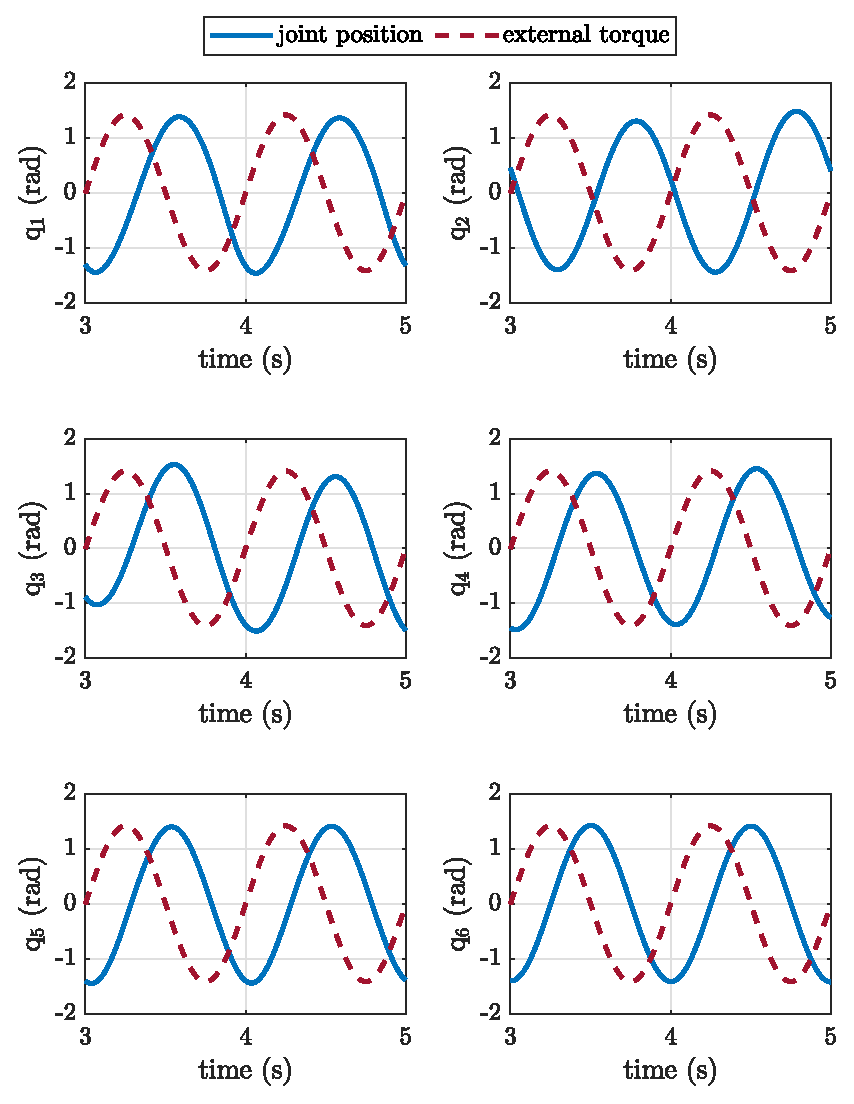
\includegraphics{joint_position_and_external_torque.eps}
\caption{Normalized joint positions ($\mathbf{q}$) and external torque ($\tauext$) with respect to time.}
\label{fig:act1.1.2_tau_and_q}
\end{figure}

\begin{figure}
\centering
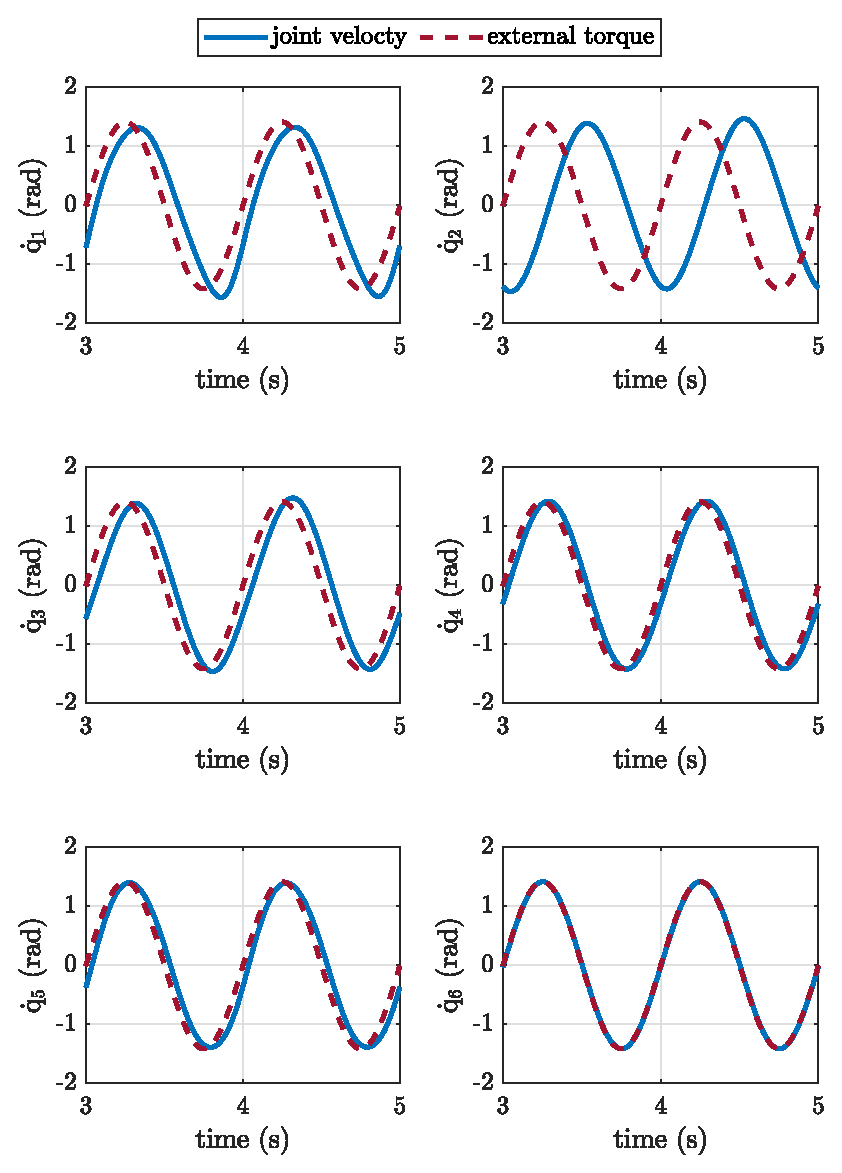
\includegraphics{joint_velocity_and_external_torque.eps}
\caption{Normalized joint velocities ($\mathbf{\dot{q}}$) and external torque ($\tauext$) with respect to time.}
\label{fig:act1.1.2_tau_and_dq}
\end{figure}

\begin{figure}
\centering
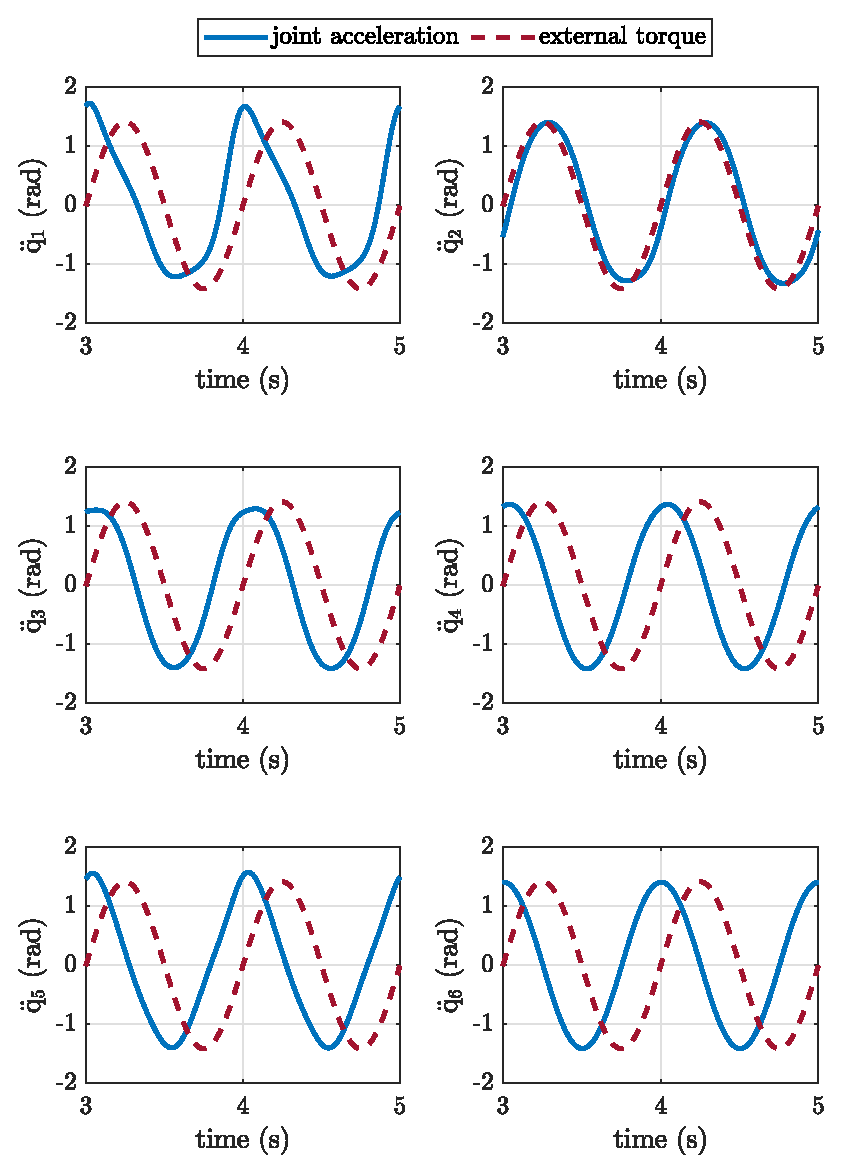
\includegraphics{joint_acceleration_and_external_torque.eps}
\caption{Normalized joint accelerations ($\mathbf{\ddot{q}}$) and external torque ($\tauext$) with respect to time.}
\label{fig:act1.1.2_tau_and_ddq}
\end{figure}
